\documentclass[12pt]{article}
\usepackage[utf8]{inputenc} % input encoding
\usepackage[T1]{fontenc} % Use an 8-bit font encoding, so that ã is a
                         % single glyph in the font. Yields better
                         % hyphenation and better cut-and-paste from pdf
\usepackage{times} % Comment this line you you want the default font, Computer Roman
% \usepackage[portuguese]{babel} % Uncomment this file you plan to write in Portuguese
\usepackage{hyperref}
\usepackage{listings}
\usepackage{graphicx}
\usepackage[section]{placeins}
\usepackage{multicol}
\usepackage{tabularx}
\usepackage{makecell}
\usepackage{amssymb}
\graphicspath{ {./images/} }
\sloppy

\lstset{frame=tb,
  aboveskip=0mm,
  belowskip=2mm,
  showstringspaces=false,
  columns=flexible,
  basicstyle={\small\ttfamily},
  numbers=none,
  breaklines=true,
  breakatwhitespace=true,
  tabsize=3
}

\title{TST JUnit Testing \\
  \Large Software Verification and Validation \\ 2019--2020
}
\author{
  João David\\49448
  \and
  Ye Yang\\49521
}
\date{09/05/2020}

\begin{document}
\maketitle
\newpage
\tableofcontents
\newpage
\section[Instruction Coverage]{Instruction Coverage}
\subsection{size()}
\begin{lstlisting}
    public int size() {
        return n; //I1
    }
\end{lstlisting}

\begin{table}[htb]
\centering
\begin{tabular}{| c | c | c | c |} 
 \hline
 Test Case & Values & Expected / Actual & IC\\ \hline
 sizeZeroTest & - & 0 & I1 \\ \hline

\end{tabular}
\end{table}

\subsection{contains(String key)}
\begin{lstlisting}
    public boolean contains(String key) {
        if (key == null)  //I1
            throw new IllegalArgumentException("argument to contains() is null"); //I2
        return get(key) != null; //I3
    }
\end{lstlisting}

\begin{table}[htb]
\centering
\begin{tabular}{| c | c | c | c |} 
 \hline
 Test Case & Values & Expected / Actual & IC\\ \hline
 containsNullKey & null & IAE & I1, I2 \\ \hline
 containsNonNullKey & "someKey" & false & I1, I3 \\ \hline
\end{tabular}
\end{table}

\subsection{get(String key)}
\begin{lstlisting}
public T get(String key) {
   if (key == null) //I1
       throw new IllegalArgumentException("calls get() with null argument"); //I2
   if (key.length() == 0) //I3
       throw new IllegalArgumentException("key must have length >= 1"); //I4
   Node<T> x = get(root, key, 0); //I5
   if (x == null) //I6
      return null; //I7
   return x.val; //I8
}
\end{lstlisting}

\begin{table}[htb]
\centering
\begin{tabular}{| c | c | c | c |} 
 \hline
 Test Case & Values & Expected / Actual & IC\\ \hline
 getNullKey & null & IAE & I1, I2 \\ \hline
 getEmptyStringKey & "" & IAE & I1, I3, I4 \\ \hline
 getNonExistentKey & “someKey” & null & I1, I3, I5, I6, I7 \\ \hline
 getExistentKey & “key” & <value> & I1, I3, I5, I6, I8 \\ \hline 
\end{tabular}
\end{table}

\subsection{put(String key, T val)}
\begin{lstlisting}
public void put(String key, T val) {
   if (key == null) //I1
      throw new IllegalArgumentException("calls put() with null key"); //I2
   if (!contains(key)) //I3
      n++; //I4
   root = put(root, key, val, 0); //I5
}
\end{lstlisting}

\begin{table}[htb]
\centering
\begin{tabular}{| c | c | c | c |} 
 \hline
 Test Case & Values & Expected / Actual & IC\\ \hline
 putNullKey & null, 1 & IAE & I1, I2 \\ \hline
 putValidNewKey & “someKey”, 1 & NoExep & I1, I3, I4, I5 \\ \hline
\end{tabular}
\end{table}


\subsection{longestPrefixOf(String query)}
\begin{lstlisting}
public String longestPrefixOf(String query) {
   if (query == null) //I1
      throw new IllegalArgumentException("calls longestPrefixOf() with null argument"); //I2
   if (query.length() == 0) //I3
      return null; //I4
   int length = 0; //I5
   Node<T> x = root; //I6
   int i = 0; //I7
   while (x != null /*I8*/ && i < query.length() /*I9*/) {
      char c = query.charAt(i); //I10
      if      (c < x.c) /*I11*/ x = x.left; //I12
      else if (c > x.c) /*I13*/ x = x.right; //I14
      else {
         i++; //I15
         if (x.val != null) //I15
            length = i; //I17
         x = x.mid; //I18
      }
   }
   return query.substring(0, length); //I19
}
\end{lstlisting}

\begin{table}[htb]
\centering
\begin{tabular}{| c | c | c | c |} 
 \hline
 Test Case & Values & Expected / Actual & IC\\ \hline
 longestPrefixOfNull & null & IAE & I1, I2 \\ \hline
 \makecell{longestPrefixOf\\EmptyString} & "" & null & I1, I3, I4 \\ \hline
 \makecell{longestPrefixOf\\AllInstructions} & "c" & "c" & \makecell{I1, I3, I5, I6,\\ I7, I8, I9, I10, \\ I11, I12, I13, I14, \\ I15, I16, I17, I18, I19} \\ \hline
\end{tabular}
\end{table}


\subsection{keys()}
\begin{lstlisting}
public Iterable<String> keys() {
   Queue<String> queue = new LinkedList<>(); //I1
   collect(root, new StringBuilder(), queue); //I2
   return queue; //I3
}
\end{lstlisting}

\begin{table}[htb]
\centering
\begin{tabular}{| c | c | c | c |} 
 \hline
 Test Case & Values & Expected / Actual & IC\\ \hline
 keysTest & - & Empty Iterator & I1, I2, I3 \\ \hline
\end{tabular}
\end{table}


\subsection{keysWithPrefix(String prefix)}
\begin{lstlisting}
public Iterable<String> keysWithPrefix(String prefix) {
    if (prefix == null) //I1
        throw new IllegalArgumentException("calls keysWithPrefix() with null argument"); //I2
    Queue<String> queue = new LinkedList<>(); //I3
    Node<T> x = get(root, prefix, 0); //I4
    if (x == null) //I5
        return queue; //I6
    if (x.val != null)  //I7
        queue.add(prefix); //I8
        collect(x.mid, new StringBuilder(prefix), queue); //I9
        return queue; //I10
}
\end{lstlisting}

\begin{table}[htb]
\centering
\begin{tabular}{| c | c | c | c |} 
 \hline
 Test Case & Values & Expected / Actual & IC\\ \hline
 keysWithPrefixNull & null & IAE & I1, I2 \\ \hline
 \makecell{keysWithPrefix\\NonExistentPrefix} & "prefix" & Iterator (size 0) & I1, I3, I4, I5, I6 \\ \hline
 \makecell{keysWithPrefix\\ExistentPrefix} & "c" & Iterator (size 1) & \makecell{I1, I3, I4, I5, \\ I6, I7, I8, I9, I10} \\ \hline
\end{tabular}
\end{table}


\subsection{keysThatMatch(String pattern)}
\begin{lstlisting}
public Iterable<String> keysThatMatch(String pattern) {
    Queue<String> queue = new LinkedList<>(); //I1
    collect(root, new StringBuilder(), 0, pattern, queue); //I2
    return queue; //I3
}
\end{lstlisting}

\begin{table}[htb]
\centering
\begin{tabular}{| c | c | c | c |} 
 \hline
 Test Case & Values & Expected / Actual & IC\\ \hline
 keysThatMatchTest & "pattern" & Iterator (size 0) & I1, I2, I3 \\ \hline
\end{tabular}
\end{table}

\subsection{delete(String key)}
\begin{lstlisting}
public void delete(String key) {
    if (key == null) { //I1
        throw new IllegalArgumentException("calls put() with null key"); //I2
    }            
    if (contains(key)) { //I3
      	n--; //I4
    	put(root, key, null, 0); //I5
    }        
}
\end{lstlisting}

\begin{table}[htb]
\centering
\begin{tabular}{| c | c | c | c |} 
 \hline
 Test Case & Values & Expected / Actual & IC\\ \hline
 deleteNull & null & IAE & I1, I2 \\ \hline
 deleteContains & "key" & Iterator (size 0) & I3, I4, I5 \\ \hline
\end{tabular}
\end{table}

\subsection{equals(Object obj)}
\begin{lstlisting}
	public boolean equals(Object obj) {
		if (this == obj) //I1
			return true; //I2
		if (obj == null) //I3
			return false; //I4
		if (!(obj instanceof TST<?>)) //I5
			return false; //I6
		
		TST<T> other = (TST<T>) obj; //I7
		if (this.size() != other.size()) { //I8
			return false; //I9
		}
			
		Iterable<String> thisIterable = this.keys(); //I10
        for(String currKey : thisIterable){ //I11
            if(!this.get(currKey).equals(other.get(currKey))){ //I12
                return false; //I13
            }
        }
		return true; //I14
	}
\end{lstlisting}

\begin{table}[htb]
\centering
\begin{tabular}{| c | c | c | c |} 
 \hline
 Test Case & Values & Expected / Actual & IC\\ \hline
 equalsSame & Same trie object & True & I1, I2 \\ \hline
 equalsNull & null & False & I1, I3, I4 \\ \hline
 equalsNotTrie & 1 & False & I1, I3, I5, I6 \\ \hline
 equalsDifSize & Trie with more keys & False & I1, I3, I5, I7, I8, I9 \\ \hline
 equalsDifContent & Trie with same keys & True & \makecell{I1, I3, I5, I7, 
 \\ I8, I10, I11, I12, I14} \\ \hline
\end{tabular}
\end{table}

\newpage
\section{Edge Coverage}

\begin{figure}[!htbp]
  	\centering
  	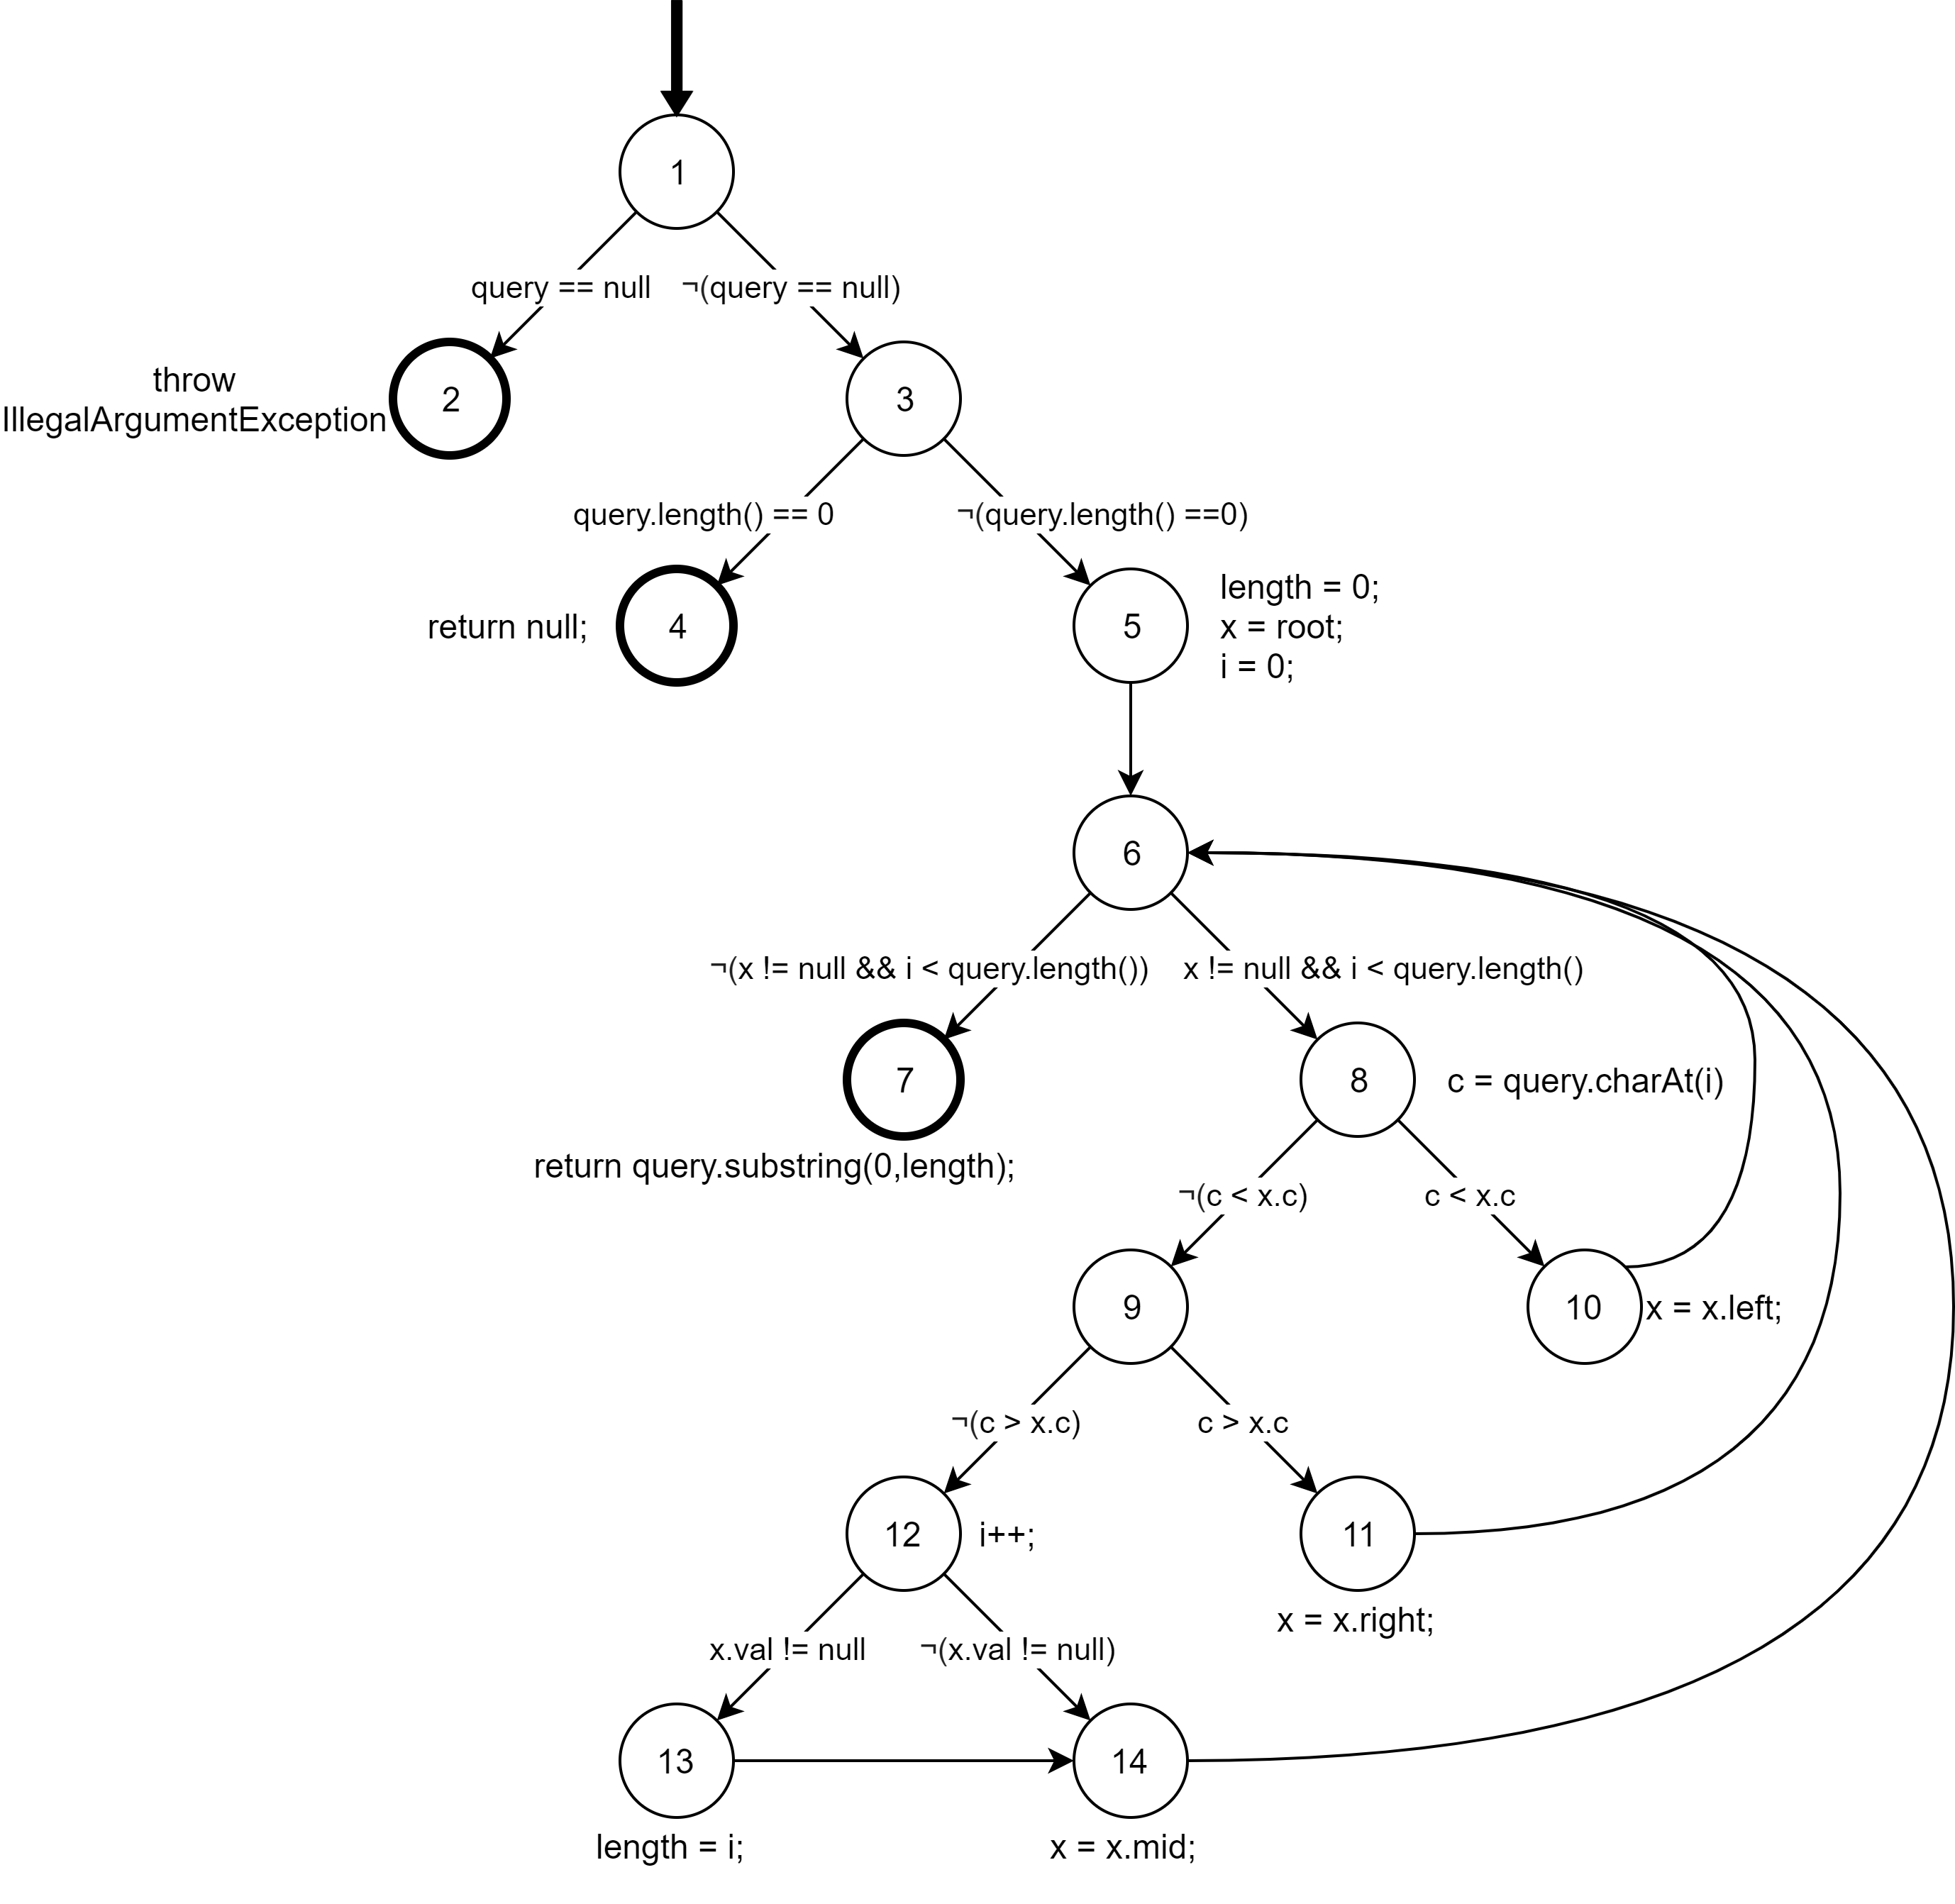
\includegraphics[scale=0.15]{longestPrefixOfGraph.png}
  	\caption{longestPrefixOf's Graph}
\end{figure}

Graph Edges: [1,2], [1,3], [3,4], [3,5], [5,6], [6,7], [6,8], [8,9], [8,10], [10,6], [9,12], [9,11], [11,6], [12,13], [12,14], [13,14], [14,6]

\newpage
\subsection{Test cases}
\begin{table}[!htbp]
\centering
\begin{tabular}{| c | c | c |} 
 \hline
 Test Case & Test Path & Edges Covered\\ \hline
 edgeCoverage1 & [1,2] & [1,2] \\ \hline
 edgeCoverage2 & [1,3,4] & [1,3] \\ \hline
 edgeCoverage3 & [1,3,5,6,8,10,6,7] & \makecell{[1,3], [3,5], [5,6], \\\ [6,8], [8,10], [10,6], [6,7]} \\ \hline
 edgeCoverage4 & [1,3,5,6,8,9,11,6,7] & \makecell{[1,3], [3,5], [5,6], [6,8],\\\ [8,9], [9,11], [11,6], [6,7]} \\ \hline
 edgeCoverage5 & [1,3,5,6,8,9,12,14,6,7] & \makecell{[1,3], [3,5], [5,6], [6,8],\\\ [8,9], [9,12], [12,14], [14,6], [6,7]} \\ \hline
 edgeCoverage6 & [1,3,5,6,8,9,12,13,14,6,7] & \makecell{[1,3], [3,5], [5,6], [6,8], [8,9],\\\ [9,12], [12,13], [13,14], [14,6], [6,7]} \\ \hline
\end{tabular}
\end{table}

\section[Prime Path Coverage]{Prime Path Coverage}
For the Prime Path Coverage, we used the graph coverage tool made available to us through the course's moodle page. With this we extracted all the possible prime paths, and all that paths needed in order to cover them, totaling 19 test cases according to the graph previously shown. All the data regarding this test coverage is shown in comments in the above indicated Java class.

\newpage
\section[All-Uses Coverage]{All-Uses Coverage}

\begin{table}[htb]
\centering
\begin{tabular}{| c | c | c |} 
 \hline
 \textbf{nodes \& edges : I} & \textbf{def(I}) & \textbf{use(I)} \\ \hline
 1                      & \{root, query\} & \{\} \\ \hline
 (1,2), (1,3)           & \{\} & \{query\} \\ \hline
 3                      & \{\} & \{\} \\ \hline
 (3,4), (3,5)           & \{\} & \{query\} \\ \hline
 4                      & \{\} & \{\} \\ \hline
 5                      & \{length, x, i\} & \{root\} \\ \hline
 (5,6)                  & \{\} & \{\} \\ \hline
 6                      & \{\} & \{\} \\ \hline
 (6,7), (6,8)           & \{\} & \{x, i, query\} \\ \hline
 7                      & \{\} & \{query, length\} \\ \hline
 8                      & \{c\} & \{i\} \\ \hline
 (8,9), (8,10)          & \{\} & \{c, x\} \\ \hline
 9                      & \{\} & \{\} \\ \hline
 10                     & \{x\} & \{x\} \\ \hline
 (10,6), (11,6), (14,6) & \{\} & \{\} \\ \hline
 (9,11), (9,12)         & \{\} & \{c, x\} \\ \hline
 12                     & \{x\} & \{x\} \\ \hline
 12                     & \{i\} & \{i\} \\ \hline
 (12,13), (12,14)       & \{\} & \{x\} \\ \hline
 13                     & \{length\} & \{i\} \\ \hline
 14                     & \{x\} & \{x\} \\ \hline
\end{tabular}
\end{table}

\begin{table}[htb]
\centering
\begin{tabular}{| c | c | c |} 
 \hline
 \textbf{var} & \textbf{node} & \textbf{du(node,var)} \\ \hline
 query        & 1 & [1,2], [1,3], [1,3,4], [1,3,5], [1,3,5,6,7], [1,3,5,6,8] \\ \hline
 root         & 1 & [1,3,5] \\ \hline
 length       & 5 & [5,6,7] \\ \cline{2-3}
	          & 13 & [13,14,6,7] \\ \hline
            & 5 & \makecell{[5,6,7], [5,6,8], [5,6,8,10], [5,6,8,9], \\\ [5,6,8,9,11]  [5,6,8,9,12], [5,6,8,9,12,13],\\\ [5,6,8,9,12,13,14], [5,6,8,9,12,14]} \\ \cline{2-3}
x            & 10 & \makecell{[10,6,7], [10,6,8], [10,6,8,10], [10,6,8,9], \\\ [10,6,8,9,11], [10,6,8,9,12], [10,6,8,9,12,13] \\\ [10,6,8,9,12,13,14], [10,6,8,9,12,14]} \\ \cline{2-3}
            & 11 & \makecell{[11,6,7], [11,6,8], [11,6,8,10], [11,6,8,9], \\\ [11,6,8,9,11], [11,6,8,9,12], [11,6,8,9,12,13] \\\ [11,6,8,9,12,13,14], [11,6,8,9,12,14]} \\ \cline{2-3}
             & 14 & \makecell{[14,6,7], [14,6,8], [14,6,8,10], [14,6,8,9] \\\ [14,6,8,9,11], [14,6,8,9,12], [14,6,8,9,12,13] \\\ [14,6,8,9,12,13,14], [14,6,8,9,12,14]} \\ \hline
 i            & 5 & [5,6,7], [5,6,8], [5,6,8,9,12], [5,6,8,9,12,13] \\ \cline{2-3}
             & 12 & \makecell{[12,13], [12,13,14,6,7], [12,13,14,6,8] \\\ [12,13,14,6,8,9,12], [12,14,6,7], \\\ [12,14,6,8], [12,14,6,8,9,12]} \\ \hline
 c            & 8 & [8,9], [8,10], [8,9,11], [8,9,12] \\ \hline
\end{tabular}
\end{table}

\begin{table}[htb]
\centering
\begin{tabular}{| c | c | c | c | c |} 
 \hline
 \textbf{Test} & \textbf{put ops} & \textbf{Values} & \textbf{Expected} & \textbf{Test Path} \\ \hline
 1             & \{\}              & null            & IAE               & [1,2]\\ \hline
 2             & \{\}              & ""              & null              & [1,3,4]\\ \hline
 3             & \{\}              & "query"         & ""                & [1,3,5,6,7]\\ \hline
 4             & \{sea\}           & "a"             & ""                & [1,3,5,6,8,10,6,7]\\ \hline
 5             & \{sea\}           & "t"             & ""                & [1,3,5,6,8,9,11,6,7]\\ \hline
 6             & \{sea, s, e, a\}  & "sea"           & "sea"             & \makecell{[1,3,5,6,8,9,12,13,14,6,8,9,\\ 12,14,6,8,9,12,13,14,6,7]}\\ \hline
 7             & \{sea, t, a\}     & "set"           & ""                & \makecell{[1,3,5,6,8,9,12,14,6,8,\\ 9,12,14,6,8,9,11,6,7]}\\ \hline
 8             & \{sea, ball, c\}  & "c"             & "c"               & \makecell{[1,3,5,6,8,10,6,8,9,11,\\ 6,8,9,12,13,14,6,7]}\\ \hline
 9             & \{sea, cat, b\}   & "b"             & "b"               & \makecell{[1,3,5,6,8,10,6,8,10,\\ 6,8,9,12,13,14,6,7]}\\ \hline
 10            & \{sea, up, w\}    & "w"             & "w"               & \makecell{[1,3,5,6,8,9,11,6,8,9,\\ 11,6,8,9,12,13,14,6,7]}\\ \hline
 11            & \{sea\}           & "sd"            & ""                & [1,3,5,6,8,9,12,14,6,8,10,6,7]\\ \hline
 12            & \{sea\}           & "su"            & ""                & [1,3,5,6,8,9,12,14,6,8,9,11,6,7]\\ \hline
 13            & \{sea, w\}        & "t"             & ""                & [1,3,5,6,8,9,11,6,8,10,6,7]\\ \hline
\end{tabular}
\end{table}


\section[Logic-based Coverage]{Logic-based Coverage}

For our Logic-based coverage we chose the Combinatorial Coverage (CoC) as it covers all the possible permutations of truth values of each clause. In order to guarantee that certain parts of the code is reached, and not only basing it off of truth values of clauses, we also added the reachability predicates from which we based our CoC off of. All the data regarding the analysis can be viewed in the Java class indicated above.

\section{Base Choice Coverage}
Given the 3 criteria, we separated them in simple blocks that would not overlap each other so as to not have any ambiguous requirements:
\begin{enumerate}
	\item \textit{Trie already includes the new key}
		\begin{itemize}
			\item Blocks : [true, false]
		\end{itemize}
	\item \textit{Trie already includes some new key prefix}
		\begin{itemize}
			\item Blocks : [true, false]
		\end{itemize}
	\item \textit{Trie is empty}
		\begin{itemize}
			\item Blocks : [true, false]
		\end{itemize}
\end{enumerate}

The chosen base choice was: \textbf{(true, true, false)} and following are all the test requirements: 
	\begin{itemize}
	 	\item (true, true, false)
	 	\item (false, true, false)
	 	\item (true, false, false)
	 	\item (true, true, true)
	\end{itemize}
	
The last test requirement \textbf{(true, true, true)} is unfeasible due to the fact that a tree can not contain a key and at the same time be empty.

The tests used to cover the test requirements can be found in the above mentioned Java source file.

\section{PIT Mutations}
Since we are only covering the longestPrefixOf() method from the TST class, the PIT Tool had to be configured to avoid creating mutants for the other methods.

In the PIT’s tab of the Run Configurations, set the following methods in the Excluded methods field:

\begin{lstlisting}
size, contains, get, put, delete, equals, keys, keysWithPrefix, collect, keysThatMatch
\end{lstlisting} 

Running every test class responsible for covering the respective coverage criteria gives the following results
\renewcommand{\labelitemi}{$\blacksquare$}
\renewcommand\labelitemii{$\square$}
 \begin{itemize}
   \item  Instruction Coverage
   \begin{itemize}
     \item {77 \% Mutation Coverage (10/13)}
     \begin{itemize}
       \item  183: changed condition boundary
	   \item  185: negated conditional
	   \item  186: negated conditional
     \end{itemize}
   \end{itemize}
   \item  Edge Coverage
   \begin{itemize}
     \item {92\% Mutation Coverage (12/13)}
     \begin{itemize}
       \item  183: changed condition boundary
     \end{itemize}
   \end{itemize}
   \item Prime Path Coverage
   \begin{itemize}
     \item {92\% Mutation Coverage (12/13)}
     \begin{itemize}
       \item  183: changed condition boundary
     \end{itemize}
   \end{itemize}
  \item All-Uses Coverage
   \begin{itemize}
     \item {92\% Mutation Coverage (12/13)}
     \begin{itemize}
       \item  183: changed condition boundary
     \end{itemize}
   \end{itemize}
   \item Logic-based test coverage
   \begin{itemize}
     \item {100\% Mutation Coverage (13/13)}
     \begin{itemize}
       \item  All mutants killed
     \end{itemize}
   \end{itemize}
 \end{itemize}


\section[JUnit QuickCheck]{JUnit QuickCheck}
In order to test the properties given, we had to create both a Trie and a String generator.

For the first property, we took all the key values from the randomly generated Trie, shuffled the keys and then inserted them back inside a new Trie. At the end we evaluate that this new Trie is equal in content to the original Trie.

For the second property, we removed all the keys from a Trie by using the implemented \textbf{delete()} function, evaluating that the size of the Trie is 0 after finishing the deletion process.

For the third property, we generated both a random Trie and a String. We then created a new Trie and inserted all the values from the original Trie plus the randomly generated String, after which we remove the same String and asserted that the final Trie is equal to the original Trie.

For the fourth and final property, we also generated a random Trie and String. The string would be inserted in portions into the Trie so that all the prefixes are inserted for later testing. For example, if we have the word \textit{generator} the following keys would be inserted into the Trie: \textit{generator}, \textit{generato}, \textit{generat}, ... , \textit{g}. After the insertion we then get all the key prefixes starting from the longest prefix to the shortest. With each prefix we test that the return of \textbf{keysWithPrefix(prefix)} from a longer (stricter prefix) is always contained inside a shorter (less strict) prefix.
\end{document}

%%% Local Variables:
%%% mode: latex
%%% TeX-master: t
%%% End:
